\documentclass[12pt]{report}
\usepackage{tikz}
\usepackage{parskip}
\usepackage{mathtools}
\usepackage{flexisym}
\usepackage{verbatim}



\begin{document}
\newcommand\tab[1][1cm]{\hspace*{#1}}

%title page
\author{Andre Gregoire}
\title{CIS770 Homework 5}
\maketitle

%problem 1
\textbf{ Problem1}\newline
\textit{1.1.} \newline 
G = (V, $\Sigma$, R, S) = ($\{S,X,Y\}$, $\{a,b\}$, R, S) \\
where R contains the transitions:
\tab S $\rightarrow$ $\{$ $\epsilon$ $\vert$ aXb $\vert$ bYa $\vert$ SS $\}$ \\
\tab X $\rightarrow$ $\{$ S $\vert$ $\epsilon$ $\}$ \\
\tab Y $\rightarrow$ $\{$ S $\vert$ $\epsilon$ $\}$ \\

\textit{1.2.}\newline
Any string w generaged by G, w $\in$ L\\
\textbf{Base case:} 1 step derivation, only one derivation contains one step and that \\ is S $\xRightarrow{*}$ $\epsilon$, thus w = $\epsilon$ so w $\in$ L \\

\textbf{Ind. Hyp:} Assume every derivation S $\xRightarrow{*}$ w, with n $\geq$ 1 steps, w $\in$ L \\

\textbf{Ind. Step:} Let S $\xRightarrow{*}$ w be a derivation with n + 1 steps, because \\ n+1 $>$ 1, the first derivation must be, aSb, bSa, SS with S being non terminal characters. \\

Case(aXb): w must be in the form a$w_1$b where $w_1$ is a string derived from non terminal S in the remaining n steps and $w_1$ $\in$ L by the inductive hypothesis. Thus w $\in$ L because by adding an a and b from the original transition to $w_1$ keeps the number of a's and b's being equivalent. \\

Case(bYa): similar to the above case, w must be in the form b$w_1$a where $w_1$ is a string derived from non terminal S in the remaining n steps and $w_1$ $\in$ L by the inductive hypothesis. Thus w $\in$ L because by adding an a and b from the original transition to $w_1$ keeps the number of a's and b's being equivalent. \\

Case(SS):  w must be in the form $w_1w_2$ where $w_1$ is a string derived from the first non terminal S and $w_2$ from the second non terminal S and $w_1$ $\in$ L, \\ 
$w_2$ $\in$ L by the inductive hypothesis, \\

Therefore every string generated by G contains an equal amount of a's and b's and exist in L. \\

\textit{1.3.}\newline

\begin{center}
	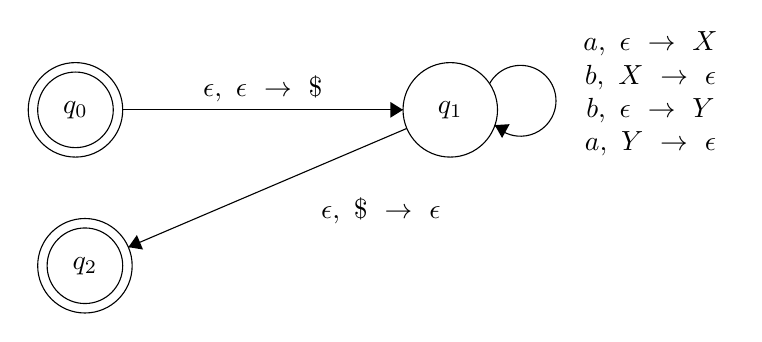
\begin{tikzpicture}[scale=0.2]
		\tikzstyle{every node}+=[inner sep=0pt]
		\draw [black] (16,-19.4) circle (3);
		\draw (16,-19.4) node {$q_0$};
		\draw [black] (16,-19.4) circle (2.4);
		\draw [black] (39.8,-19.4) circle (3);
		\draw (39.8,-19.4) node {$q_1$};
		\draw [black] (16.6,-29.3) circle (3);
		\draw (16.6,-29.3) node {$q_2$};
		\draw [black] (16.6,-29.3) circle (2.4);
		\draw [black] (42.289,-17.746) arc (151.33474:-136.66526:2.25);
		\draw (47.17,-18.4) node [right] {\begin{tabular}{c}$a,\mbox{ }\epsilon\mbox{ }\rightarrow\mbox{ }X$\\ $b,\mbox{ }X\mbox{ }\rightarrow\mbox{ }\epsilon$\\ $b,\mbox{ }\epsilon\mbox{ }\rightarrow\mbox{ }Y$ \\ $a,\mbox{ }Y\mbox{ }\rightarrow\mbox{ }\epsilon$\end{tabular}};
		\fill [black] (42.63,-20.37) -- (43.09,-21.19) -- (43.57,-20.31);
		\draw [black] (19,-19.4) -- (36.8,-19.4);
		\fill [black] (36.8,-19.4) -- (36,-18.9) -- (36,-19.9);
		\draw (27.9,-18.9) node [above] {$\epsilon,\mbox{ }\epsilon\mbox{ }\rightarrow\mbox{ }\$$};
		\draw [black] (37.04,-20.58) -- (19.36,-28.12);
		\fill [black] (19.36,-28.12) -- (20.29,-28.27) -- (19.9,-27.35);
		\draw (35.39,-24.94) node [below] {$\epsilon, \mbox{ }\$\mbox{ }\rightarrow\mbox{ }\epsilon$};
	\end{tikzpicture}
\end{center}


To build the PDA I just stepped through the CFG.  It is in an accepting state when the string is empty thus the initial state is an accepting state because there is an equal number of a's and b's and the stack is empty.  After we push our initial symbol, in this case '\$' we start reading in characters from the string and pop/push to the stack accordingly.  If we read an 'a' and there is a non-terminal 'Y' on the top of the stack we pop it and push nothing.  This is denote a pair of a and b's in the string so each pair makes up a single 'a' and a single 'b' this is to keep track of the number of a's and b's we've read in.  if there is not a non-terminal Y on the top of the stack we push a non-terminal X to the stack.  Similar to 'a' if we read a 'b' and there is a non-terminal X on the top of the stack we push nothing because we found a pair, and if there is not a non-terminal X we push a non-terminal Y to hopefully find a matching 'a' to pop it from the stack.  If the string in question does exist in our language the final character in the stack should be our initial push '\$' and we can pop it and go back to the accepting state.

P = (Q, $\Sigma$, $\Gamma$, $\delta$, $q_0$, F)\\
\tab Q = \{$q_0$, $q_1$, $q_2$\}\\
\tab $\Gamma$ = V $\cup$ $\Sigma$ $\cup$ \{\$\} where \$ $\notin$ V $\cup$ $\Sigma$\\
\tab $q_0$ = $q_0$\\
\tab F = \{$q_0$, $q_2$\}\\
\tab $\delta$ transitions \\
\tab\tab $\delta$($q_0, \epsilon, \epsilon$) = \{($q_1, \$$)\}
\tab\tab $\delta$($q_1, a, \epsilon$) = \{($q_1, X$)\}\\
\tab\tab $\delta$($q_1, b, X$) = \{($q_1, \epsilon$)\}
\tab\tab $\delta$($q_1, b, \epsilon$) = \{($q_1, Y$)\}\\
\tab\tab $\delta$($q_1, a, Y$) = \{($q_1, \epsilon$)\}
\tab\tab $\delta$($q_1, \epsilon, \$$) = \{($q_2, \epsilon$)\}\\



\textbf{ Problem2}\newline
\textit{2.1.}
G = (V, $\Sigma$, R, S) = ($\{S,X,Y,R,T\}$, $\{a,b,c\}$, R, S) \\
where R contains the transitions:\\
\tab S $\rightarrow$ X $\vert$ Y\\
\tab X $\rightarrow$ Xc $\vert$ R\\
\tab Y $\rightarrow$ aY $\vert$ T\\
\tab R $\rightarrow$ aRb $\vert$ $\epsilon$\\
\tab T $\rightarrow$ bTc $\vert$ $\epsilon$\\

Yes this grammar is ambiguous because a single string can be generated from multiple transition paths, such as 'abc'.  You can obtain 'abc' by starting in either of the starting transitions (S $\rightarrow$ X $\vert$ Y). i.e. \\
\tab S $\Rightarrow$ U $\Rightarrow$ aU $\Rightarrow$ aX $\Rightarrow$  abXc $\Rightarrow$ ab$\epsilon$c = abc \\
\tab S $\Rightarrow$ V $\Rightarrow$ Vc $\Rightarrow$ Yc $\Rightarrow$ aYbc $\Rightarrow$ a$\epsilon$bc = abc \\


\pagebreak
\textbf{ Extra Credit}\newline

\begin{comment}
\begin{center}
	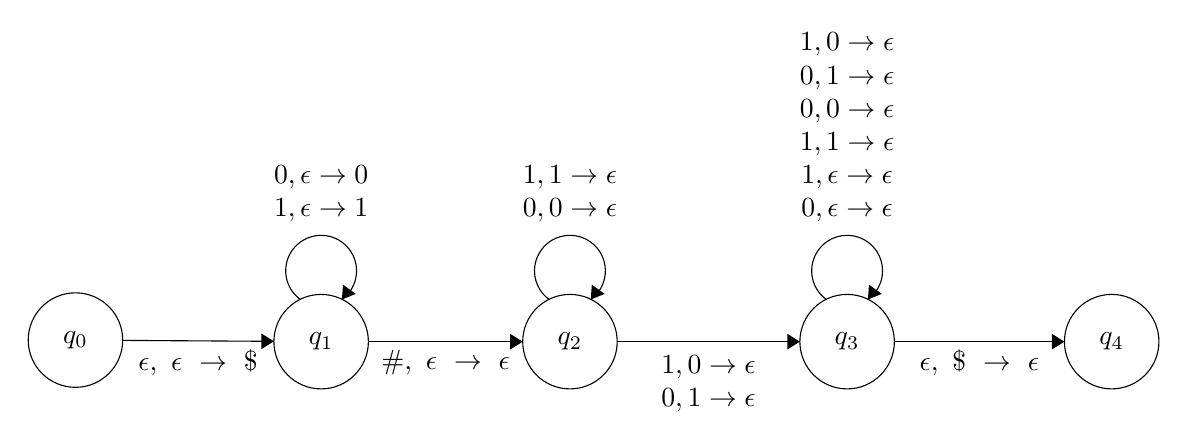
\begin{tikzpicture}[scale=0.2]
		\tikzstyle{every node}+=[inner sep=0pt]
		\draw [black] (6.1,-17.2) circle (3);
		\draw (6.1,-17.2) node {$q_0$};
		\draw [black] (21.7,-17.3) circle (3);
		\draw (21.7,-17.3) node {$q_1$};
		\draw [black] (37.5,-17.3) circle (3);
		\draw (37.5,-17.3) node {$q_2$};
		\draw [black] (55.1,-17.3) circle (3);
		\draw (55.1,-17.3) node {$q_3$};
		\draw [black] (71.9,-17.3) circle (3);
		\draw (71.9,-17.3) node {$q_4$};
		\draw [black] (9.1,-17.22) -- (18.7,-17.28);
		\fill [black] (18.7,-17.28) -- (17.9,-16.78) -- (17.9,-17.78);
		\draw (13.89,-17.8) node [below] {$\epsilon,\mbox{ }\epsilon\mbox{ }\rightarrow\mbox{ }\$$};
		\draw [black] (24.7,-17.3) -- (34.5,-17.3);
		\fill [black] (34.5,-17.3) -- (33.7,-16.8) -- (33.7,-17.8);
		\draw (29.6,-17.8) node [below] {$\#,\mbox{ }\epsilon\mbox{ }\rightarrow\mbox{ }\epsilon$};
		\draw [black] (40.5,-17.3) -- (52.1,-17.3);
		\fill [black] (52.1,-17.3) -- (51.3,-16.8) -- (51.3,-17.8);
		\draw (46.3,-17.8) node [below] {\begin{tabular}{c}$1, 0 \rightarrow \epsilon$\\ $0, 1 \rightarrow \epsilon $\end{tabular}};
		\draw [black] (58.1,-17.3) -- (68.9,-17.3);
		\fill [black] (68.9,-17.3) -- (68.1,-16.8) -- (68.1,-17.8);
		\draw (63.5,-17.8) node [below] {$\epsilon,\mbox{ }\$\mbox{ }\rightarrow\mbox{ }\epsilon$};
		\draw [black] (20.377,-14.62) arc (234:-54:2.25);
		\draw (21.7,-10.05) node [above] {\begin{tabular}{c}$ 0, \epsilon \rightarrow 0$ \\ $1, \epsilon \rightarrow 1$\end{tabular}};
		\fill [black] (23.02,-14.62) -- (23.9,-14.27) -- (23.09,-13.68);
		\draw [black] (36.177,-14.62) arc (234:-54:2.25);
		\draw (37.5,-10.05) node [above] {\begin{tabular}{c}$1, 1 \rightarrow \epsilon$ \\ $0, 0 \rightarrow \epsilon $\end{tabular}};
		\fill [black] (38.82,-14.62) -- (39.7,-14.27) -- (38.89,-13.68);
		\draw [black] (53.777,-14.62) arc (234:-54:2.25);
		\draw (55.1,-10.05) node [above] {\begin{tabular}{c}$1, 0 \rightarrow \epsilon$ \\ $0, 1 \rightarrow \epsilon$ \\ $0, 0 \rightarrow \epsilon$ \\ $1, 1 \rightarrow \epsilon$\\ $1, \epsilon \rightarrow \epsilon$\\ $0, \epsilon \rightarrow \epsilon $\end{tabular}};
		\fill [black] (56.42,-14.62) -- (57.3,-14.27) -- (56.49,-13.68);
	\end{tikzpicture}
\end{center}

\begin{flushleft} 
	I noticed after making it, this only works if x $\neq$ y, if y = x\textsuperscript{R}.  So if it wasn't palindrome, a reworked version is below.
\end{flushleft}

\begin{flushleft}
	To begin, we push our starting symbol, I used '\$'.  We then read the string value for x, from the word x\#y. this is done in $q_1$.  While reading the input from the string x we push each value onto the stack, this is used later to determine if x = y.  After we read the '\#' we move onto the next state that beings reading 'y'.  Unlike when we read in 'x' we want to now pop values that are the same as what we are reading, if we read a 1, and pop a 1 we stay in this state ($q_2$), however if a character differs we move onto a state that we can later  move onto an accepting state after we clear the stack.
\end{flushleft}

P = (\{$q_0, q_1, q_2, q_3, q_4$\}, \{0,1\}, $\Gamma$, $\delta$, $q_0$, \{$q_0$\}) where: \\
\tab $\Gamma$ = V $\cup$ $\Sigma$ $\cup$ \{\$\} where \$ $\notin$ V $\cup$ $\Sigma$ \\
\tab transitions: \\
\tab\tab $\delta(q_0, \epsilon, \epsilon) = \{(q_1,  \$)$\}
\tab\tab $\delta(q_1, 0, \epsilon) = \{(q_1,  0)$\}\\
\tab\tab $\delta(q_1, 1, \epsilon) = \{(q_1,  1)$\}
\tab\tab $\delta(q_1, \#, \epsilon) = \{(q_2,  \epsilon)$\}\\
\tab\tab $\delta(q_2, 1, 1) = \{(q_2,  \epsilon)$\}
\tab\tab $\delta(q_2, 0, 0) = \{(q_2,  \epsilon)$\}\\
\tab\tab $\delta(q_2, 1, 0) = \{(q_3,  \epsilon)$\}
\tab\tab $\delta(q_2, 0, 1) = \{(q_3,  \epsilon)$\}\\
\tab\tab $\delta(q_3, 0, 0) = \{(q_3,  \epsilon)$\}
\tab\tab $\delta(q_3, 0, 1) = \{(q_3,  \epsilon)$\}\\
\tab\tab $\delta(q_3, 0, \epsilon) = \{(q_3,  \epsilon)$\}
\tab\tab $\delta(q_3, 1, 1) = \{(q_3,  \epsilon)$\}\\
\tab\tab $\delta(q_3, 1, 0) = \{(q_3,  \epsilon)$\}
\tab\tab $\delta(q_3, 1, \epsilon) = \{(q_3,  \epsilon)$\}\\
\tab\tab $\delta(q_3, \epsilon, \$) = \{(q_4,  \epsilon)$\}\\

\end{comment}

\begin{center}
	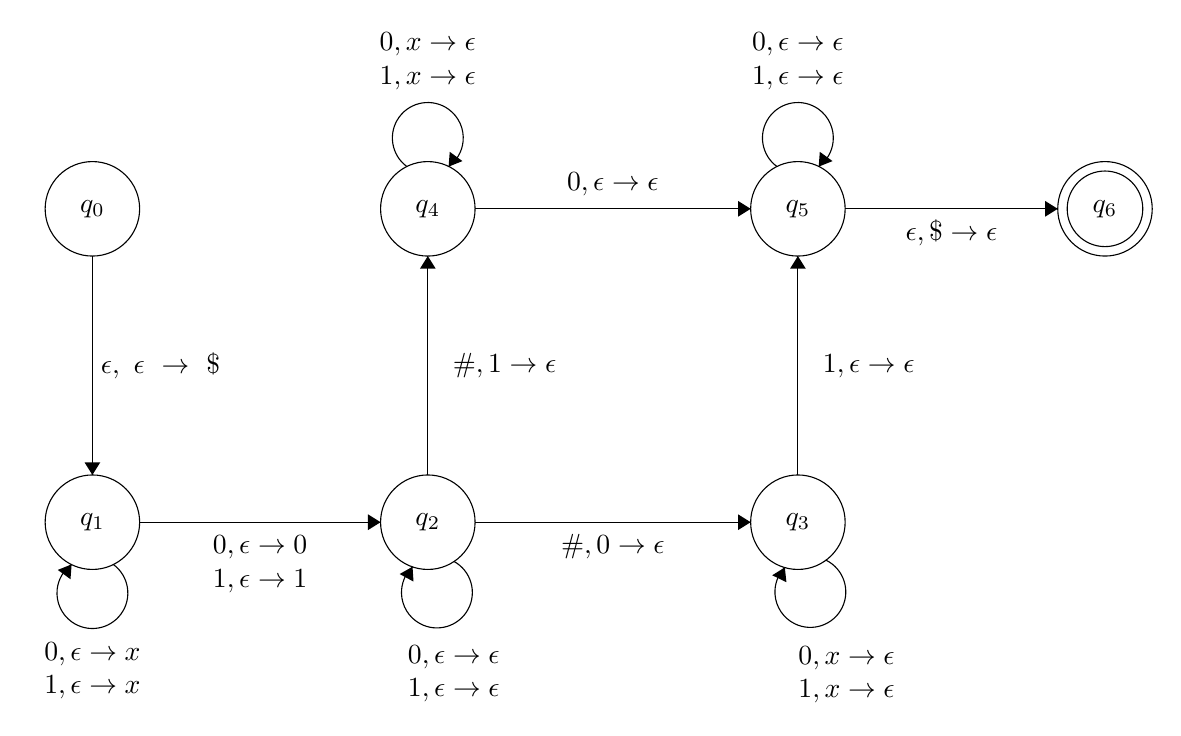
\begin{tikzpicture}[scale=0.2]
		\tikzstyle{every node}+=[inner sep=0pt]
		\draw [black] (6.6,-16.2) circle (3);
		\draw (6.6,-16.2) node {$q_0$};
		\draw [black] (6.6,-36.1) circle (3);
		\draw (6.6,-36.1) node {$q_1$};
		\draw [black] (27.9,-36.1) circle (3);
		\draw (27.9,-36.1) node {$q_2$};
		\draw [black] (27.9,-16.2) circle (3);
		\draw (27.9,-16.2) node {$q_4$};
		\draw [black] (51.4,-16.2) circle (3);
		\draw (51.4,-16.2) node {$q_5$};
		\draw [black] (51.4,-36.1) circle (3);
		\draw (51.4,-36.1) node {$q_3$};
		\draw [black] (70.9,-16.2) circle (3);
		\draw (70.9,-16.2) node {$q_6$};
		\draw [black] (70.9,-16.2) circle (2.4);
		\draw [black] (6.6,-19.2) -- (6.6,-33.1);
		\fill [black] (6.6,-33.1) -- (7.1,-32.3) -- (6.1,-32.3);
		\draw (7.1,-26.15) node [right] {$\epsilon,\mbox{ }\epsilon\mbox{ }\rightarrow\mbox{ }\$$};
		\draw [black] (9.6,-36.1) -- (24.9,-36.1);
		\fill [black] (24.9,-36.1) -- (24.1,-35.6) -- (24.1,-36.6);
		\draw (17.25,-36.6) node [below] {\begin{tabular}{c}$0, \epsilon \rightarrow 0$\\ $1, \epsilon \rightarrow 1$ \end{tabular}};
		\draw [black] (27.9,-33.1) -- (27.9,-19.2);
		\fill [black] (27.9,-19.2) -- (27.4,-20) -- (28.4,-20);
		\draw (28.4,-26.15) node [right] {\begin{tabular}{c}$\#, 1 \rightarrow \epsilon$ \end{tabular}};
		\draw [black] (30.9,-16.2) -- (48.4,-16.2);
		\fill [black] (48.4,-16.2) -- (47.6,-15.7) -- (47.6,-16.7);
		\draw (39.65,-15.7) node [above] {\begin{tabular}{c}$0, \epsilon \rightarrow \epsilon$ \end{tabular}};
		\draw [black] (7.923,-38.78) arc (54:-234:2.25);
		\draw (6.6,-43.35) node [below] {\begin{tabular}{c}$0, \epsilon \rightarrow x$\\ $1, \epsilon \rightarrow x$ \end{tabular}};
		\fill [black] (5.28,-38.78) -- (4.4,-39.13) -- (5.21,-39.72);
		\draw [black] (29.555,-38.588) arc (61.36834:-226.63166:2.25);
		\draw (29.55,-43.54) node [below] {\begin{tabular}{c}$0, \epsilon \rightarrow \epsilon$\\$1, \epsilon \rightarrow \epsilon$ \end{tabular}};
		\fill [black] (26.93,-38.93) -- (26.11,-39.39) -- (26.99,-39.87);
		\draw [black] (26.577,-13.52) arc (234:-54:2.25);
		\draw (27.9,-8.95) node [above] {\begin{tabular}{c}$0, x \rightarrow \epsilon$\\ $1, x \rightarrow \epsilon$ \end{tabular}};
		\fill [black] (29.22,-13.52) -- (30.1,-13.17) -- (29.29,-12.58);
		\draw [black] (30.9,-36.1) -- (48.4,-36.1);
		\fill [black] (48.4,-36.1) -- (47.6,-35.6) -- (47.6,-36.6);
		\draw (39.65,-36.6) node [below] {\begin{tabular}{c}$\#, 0 \rightarrow \epsilon$  \end{tabular}};
		\draw [black] (51.4,-33.1) -- (51.4,-19.2);
		\fill [black] (51.4,-19.2) -- (50.9,-20) -- (51.9,-20);
		\draw (51.9,-26.15) node [right] {\begin{tabular}{c}$1, \epsilon \rightarrow \epsilon$ \end{tabular}};
		\draw [black] (54.4,-16.2) -- (67.9,-16.2);
		\fill [black] (67.9,-16.2) -- (67.1,-15.7) -- (67.1,-16.7);
		\draw (61.15,-16.7) node [below] {\begin{tabular}{c}$\epsilon, \$ \rightarrow \epsilon$ \end{tabular}};
		\draw [black] (53.173,-38.505) arc (64.12467:-223.87533:2.25);
		\draw (54.49,-43.61) node [below] {\begin{tabular}{c}$0, x \rightarrow \epsilon$\\$1, x \rightarrow \epsilon$ \end{tabular}};
		\fill [black] (50.57,-38.97) -- (49.77,-39.47) -- (50.67,-39.91);
		\draw [black] (50.077,-13.52) arc (234:-54:2.25);
		\draw (51.4,-8.95) node [above] {\begin{tabular}{c}$0, \epsilon \rightarrow \epsilon$\\ $ 1, \epsilon \rightarrow \epsilon$ \end{tabular}};
		\fill [black] (52.72,-13.52) -- (53.6,-13.17) -- (52.79,-12.58);
	\end{tikzpicture}
\end{center}

\begin{flushleft}
	We begin by pushing the start symbol (\$) and we need to make sure the strings x and y are not equal.  So there is some character in a random position i such that $x_i \neq y_i$.  We will push filler symbols(\textit{x}) onto the stack until this random position is chosen and place this value on the stack.  This value determines which path we choose when branch out after reading in the middle character(\#).  In both paths the filler values are popped and if we reach the end of the placeholders and the next value is different then $x_i$ value used to determine our branched path it moves to the next state to finish reading the string and move onto the accepting state, however if they are the same the current thread is stuck and is thus not accepted.
\end{flushleft}

\pagebreak

\textbf{Formal Definition}, I don't think this was necessary but if something about how i denoted this was wrong please let me know.\\

P = (Q, $\Sigma$, $\Gamma$, $\delta$, $q_0$, F) where: \\
\tab Q = \{$q_0, q_1, q_2, q_3, q_4, q_5, q_6$\}\\
\tab $\Sigma$ = \{0,1\}\\
\tab $\Gamma$ = V $\cup$ $\Sigma$ $\cup$ \{\$, x\} where \$, x $\notin$ V $\cup$ $\Sigma$ \\
\tab $q_0$ = $q_0$\\
\tab F = \{$q_0, q_6$\}\\
\tab Transitions($\delta$): \\
\begin{equation*}
	\begin{aligned}[c]
		\delta(q_0, \epsilon, \epsilon) = \{(q_1,  \$)\} \\
		\delta(q_1, 0, \epsilon) = \{(q_1,  x)\}         \\
		\delta(q_1, 1, \epsilon) = \{(q_1,  x)\}         \\
		\delta(q_1, 0, \epsilon) = \{(q_2,  0)\}         \\
		\delta(q_1, 1, \epsilon) = \{(q_2,  1)\}         \\
		\delta(q_2, 0, \epsilon) = \{(q_2,  \epsilon)\}  \\
		\delta(q_2, 1, \epsilon) = \{(q_2,  \epsilon)\}  \\
		\delta(q_2, \#, 1) = \{(q_4,  \epsilon)\}        \\
		\delta(q_2, \#, 0) = \{(q_3,  \epsilon)\}        \\
	\end{aligned}
	\quad\quad
	\begin{aligned}[c]
		\delta(q_3, 0, x) = \{(q_3,  \epsilon)\}         \\
		\delta(q_3, 1, x) = \{(q_3,  \epsilon)\}         \\
		\delta(q_3, 1, \epsilon) = \{(q_5,  \epsilon)\}  \\
		\delta(q_4, 0, x) = \{(q_3,  \epsilon)\}         \\
		\delta(q_4, 1, x) = \{(q_3,  \epsilon)\}         \\
		\delta(q_4, 0, \epsilon) = \{(q_5,  \epsilon)\}  \\
		\delta(q_5, 0, \epsilon) = \{(q_5,  \epsilon)\}  \\
		\delta(q_5, 1, \epsilon) = \{(q_5,  \epsilon)\}  \\
		\delta(q_5, \epsilon, \$) = \{(q_6,  \epsilon)\} \\
	\end{aligned}
\end{equation*}


Note: Is there such thing as a pda with more than one stack? My original idea for this problem ended up requiring a second stack but I was unsure if it was possible.\\

\end{document}
